% Options for packages loaded elsewhere
\PassOptionsToPackage{unicode}{hyperref}
\PassOptionsToPackage{hyphens}{url}
%
\documentclass[
  a4paper,
]{article}
\usepackage{amsmath,amssymb}
\usepackage{setspace}
\usepackage{iftex}
\ifPDFTeX
  \usepackage[T1]{fontenc}
  \usepackage[utf8]{inputenc}
  \usepackage{textcomp} % provide euro and other symbols
\else % if luatex or xetex
  \usepackage{unicode-math} % this also loads fontspec
  \defaultfontfeatures{Scale=MatchLowercase}
  \defaultfontfeatures[\rmfamily]{Ligatures=TeX,Scale=1}
\fi
\usepackage{lmodern}
\ifPDFTeX\else
  % xetex/luatex font selection
\fi
% Use upquote if available, for straight quotes in verbatim environments
\IfFileExists{upquote.sty}{\usepackage{upquote}}{}
\IfFileExists{microtype.sty}{% use microtype if available
  \usepackage[]{microtype}
  \UseMicrotypeSet[protrusion]{basicmath} % disable protrusion for tt fonts
}{}
\makeatletter
\@ifundefined{KOMAClassName}{% if non-KOMA class
  \IfFileExists{parskip.sty}{%
    \usepackage{parskip}
  }{% else
    \setlength{\parindent}{0pt}
    \setlength{\parskip}{6pt plus 2pt minus 1pt}}
}{% if KOMA class
  \KOMAoptions{parskip=half}}
\makeatother
\usepackage{xcolor}
\usepackage[margin=1in]{geometry}
\usepackage{graphicx}
\makeatletter
\def\maxwidth{\ifdim\Gin@nat@width>\linewidth\linewidth\else\Gin@nat@width\fi}
\def\maxheight{\ifdim\Gin@nat@height>\textheight\textheight\else\Gin@nat@height\fi}
\makeatother
% Scale images if necessary, so that they will not overflow the page
% margins by default, and it is still possible to overwrite the defaults
% using explicit options in \includegraphics[width, height, ...]{}
\setkeys{Gin}{width=\maxwidth,height=\maxheight,keepaspectratio}
% Set default figure placement to htbp
\makeatletter
\def\fps@figure{htbp}
\makeatother
\setlength{\emergencystretch}{3em} % prevent overfull lines
\providecommand{\tightlist}{%
  \setlength{\itemsep}{0pt}\setlength{\parskip}{0pt}}
\setcounter{secnumdepth}{-\maxdimen} % remove section numbering
\ifLuaTeX
\usepackage[bidi=basic]{babel}
\else
\usepackage[bidi=default]{babel}
\fi
\babelprovide[main,import]{catalan}
% get rid of language-specific shorthands (see #6817):
\let\LanguageShortHands\languageshorthands
\def\languageshorthands#1{}
\ifLuaTeX
  \usepackage{selnolig}  % disable illegal ligatures
\fi
\usepackage{bookmark}
\IfFileExists{xurl.sty}{\usepackage{xurl}}{} % add URL line breaks if available
\urlstyle{same}
\hypersetup{
  pdftitle={U2. Windows Server. Instal·lació i ús},
  pdfauthor={@tofermos 2024},
  pdflang={ca-ES},
  hidelinks,
  pdfcreator={LaTeX via pandoc}}

\title{U2. Windows Server. Instal·lació i ús}
\author{@tofermos 2024}
\date{}

\begin{document}
\maketitle

{
\setcounter{tocdepth}{2}
\tableofcontents
}
\setstretch{1.5}
\newpage
\renewcommand\tablename{Tabla}

\section{1. Introducció a Windows
Server}\label{introducciuxf3-a-windows-server}

Windows Server és un sistema operatiu desenvolupat per Microsoft,
dissenyat per a administrar xarxes, emmagatzematge i aplicacions a
nivell empresarial, allotjament de llocs web, gestió de bases de dades i
centralització de recursos compartits.

Algunes de les principals característiques de Windows Server inclouen:

\begin{itemize}
\item
  \textbf{Active Directory}: Un \emph{servei de directori} que permet la
  gestió d'usuaris, equips i polítiques de seguretat en la xarxa de
  forma centralitzada.
\item
  \textbf{Hyper-V}: Tecnologia de virtualització integrada que permet
  crear i administrar màquines virtuals.
\item
  \textbf{IIS (Internet Information Services)}: Plataforma per a
  allotjar aplicacions web. Pemet que el servidor siga un servidor web.
\item
  \textbf{Administració de servidors}: A través d'eines com
  l'Administrador de Servidors, es poden gestionar múltiples rols i
  funcions del servidor.
\end{itemize}

\section{2. Instal·lació en un equip
informàtic}\label{installaciuxf3-en-un-equip-informuxe0tic}

Abans d'utilitzar Windows Server, és essencial entendre el procés
d'instal·lació, que consta de diversos passos tècnics importants. No
obstant, no són molt diferents al ja vistos en un Windows 1x. Ens
centrem en repassar allò més important.

\subsection{2.1 Particions i sistemes
d'arxius}\label{particions-i-sistemes-darxius}

\subsubsection{Particions}\label{particions}

Són divisions del disc dur on s'emmagatzemarà el sistema operatiu o les
dades. Durant la instal·lació de Windows Server (com la de qualsevol
SO), cal triar com particionar el disc.

\begin{quote}
Nota:

En un servidor hem de separar les dades de la instal·lació del SO.
\end{quote}

\subsubsection{Taula de particions}\label{taula-de-particions}

Tenim dos possibilitats la més antiga \textbf{MBR (Master Boot Record)}
i la més moderna hui en dia ja generalitzada \textbf{GPT} que é sla que
usarem.

\textbf{MBR (Master Boot Record)}

\begin{itemize}
\tightlist
\item
  \textbf{Nombre màxim de particions:} 4 particions primàries.
\end{itemize}

Si es necessita més de 4 particions, es poden tenir 3 particions
primàries i 1 partició estesa, dins la qual es poden crear múltiples
particions lògiques.

\begin{itemize}
\item
  \textbf{Tipus de particions:}

  \begin{itemize}
  \item
    \textbf{Primàries:} Particions directament accessibles pel sistema
    operatiu (màxim 4).
  \item
    \textbf{Estesa:} Una partició que pot contenir particions lògiques.
  \item
    \textbf{Lògiques:} Particions dins de la partició estesa.
  \end{itemize}
\item
  \textbf{Tamany màxim del disc}: 2 TB (terabytes), el MBR utilitza 32
  bits per adreçar sectors de 512 Bytes.
\end{itemize}

\subsubsection{GPT (GUID Partition
Table)}\label{gpt-guid-partition-table}

\begin{itemize}
\tightlist
\item
  \textbf{Nombre màxim de particions:} Teòricament il·limitat, però
  pràcticament uns 128 en la majoria de sistemes operatius.
\item
  \textbf{Tipus de particions:} Totes les particions són
  \textbf{primàries}, no hi ha limitació d'estesa o lògiques com en MBR.
\item
  \textbf{Nombre màxim de particions:} Teòricament il·limitat, però
  pràcticament uns 128 en la majoria de sistemes operatius.
\item
  \textbf{Tipus de particions:}

  \begin{itemize}
  \tightlist
  \item
    Totes les particions són \textbf{primàries}
  \end{itemize}
\item
  \textbf{Tamany màxim del disc} 9.4 ZB (zettabytes) teòrics.GPT
  utilitza un esquema d'adreces de 64 bits
\end{itemize}

\subsubsection{Sistema d'arxius.}\label{sistema-darxius.}

Windows Server utilitza principalment el sistema \textbf{NTFS (New
Technology File System)}, que ofereix millores respecte a FAT32. Les dos
primeres superen les limitacions vistes al curs anterior de particions
de 32GBytes i fitxers de 4GBytes de FAT32:

\begin{enumerate}
\def\labelenumi{\arabic{enumi}.}
\item
  \textbf{Suport per a fitxers grans:} NTFS admet fitxers de fins a 16
  TB, mentre que FAT32 està limitat a 4 GB per fitxer.
\item
  \textbf{Tamany màxim de partició:} NTFS suporta particions de fins a
  256 TB, mentre que FAT32 es limita a 32 GB (en Windows).
\item
  \textbf{Seguretat i permisos:} NTFS permet assignar permisos d'accés
  més detallats que el simple Lectura/Escriptura/Control Total a fitxers
  i carpetes.
\item
  \textbf{Encriptació (EFS - Encrypting File System):}. Permet xifrar
  fitxers i carpetes individualment, mantenint-lo protegit davant accés
  no autoritzat. És una encriptació transparent per a l'usuari
  autoritzat (pot accedir-hi sense desxifrar manualment els fitxers)
  mentre que altres usuaris o sistemes no.
\item
  \textbf{Compressió (NTFS Compression):} Compressió nativa i
  transparent: els fitxers i carpetes es poden utilitzar normalment
  sense necessitat de descomprimir-los manualment. Penalitza molt poc el
  rendiment: molt útil si tenim fitxers que usem poc i més si tenen prou
  tamany.
\item
  \textbf{Recuperació d'errors:} NTFS registra les transaccions
  (journaling) i pot recuperar-se automàticament d'alguns errors del
  sistema, cosa que FAT32 no fa.
\end{enumerate}

7 \textbf{Quotes de discs} Suposa poder limitar l'espai de disc per als
usuaris. Ho practicarem en properes unitats.

8 \textbf{Fragmentació:} NTFS gestiona millor la fragmentació de dades
en disc en comparació amb FAT32.

\textbf{ReFS (Resilient File System)} Tot i que NTFS és l'estàndard,
sobretot per a la partició de sistema, ReFS es un sistema més nou per a
servidores con alta resiliència a errors.

Al present curs anem a treballar amb NTFS.

\subsection{Recomanacions generals}\label{recomanacions-generals}

\begin{enumerate}
\def\labelenumi{\arabic{enumi}.}
\tightlist
\item
  Usar GPT.
\item
  Separar en discos durs distints la instal·lació del SO de la resta de
  dades.
\item
  Si només tenim un disc (o conjunt que implementes una unitat tipus
  RAID), crearem particions distintes.
\item
  Si, pot ser, les crearem en el procés d'intal·lació o, almenys, abans
  de començar a operar. En cas contrari, hem de fer còpia de seguretat
  de les dades abans de reparticionar discos.
\item
  Si tenim discos de distint rendiment (SSD i HDD), és preferible que el
  SO i les aplicacions més utilitzades estiguen instal·lades al disc més
  ràpid.
\item
  Tant el backup com els sistemes de redundància són fonamentals. També
  les snapshots. (Els veiem més avant)
\end{enumerate}

\subsection{2.2 Gestors d'arrancada}\label{gestors-darrancada}

El gestor d'arrancada és un programari que s'encarrega d'iniciar el
sistema operatiu durant el procés d'arrancada de l'equip.

\begin{itemize}
\tightlist
\item
  \textbf{Windows Boot Manager} és el gestor d'arrancada predeterminat
  de Windows Server. Aquest programari s'encarrega de gestionar el
  procés d'arrancada del sistema i, en cas d'haver-hi diversos sistemes
  operatius instal·lats en l'equip, permet seleccionar quin iniciar.
\end{itemize}

\subsection{2.3 Procés d'instal·lació}\label{procuxe9s-dinstallaciuxf3}

El procés d'instal·lació de Windows Server és similar al de les versions
d'escriptori de Windows, però amb alguns passos addicionals per a la
configuració de rols i característiques del servidor. Els passos
generals inclouen:

\begin{enumerate}
\def\labelenumi{\arabic{enumi}.}
\tightlist
\item
  \textbf{Preparar l'equip}: Comprovar els requisits de maquinari, com
  CPU, RAM i espai en disc.
\item
  \textbf{Arrancada des del mitjà d'instal·lació}: Açò pot ser des d'un
  DVD o una unitat USB bootable. Al VirtualBox usarem la unitat òptica.
\item
  \textbf{Selecció de la partició}: Triar la unitat o partició on
  s'instal·larà Windows Server.
\item
  \textbf{Configuració inicial}: Assignar un nom al servidor, configurar
  la xarxa i el compte d'administrador. Serà administrador de tota la
  xarxa com vorem.
\item
  \textbf{Configuració de rols}: Durant o després de la instal·lació, es
  poden afegir rols al servidor. El més important és el de controlador
  de domini però hi ha altres.
\end{enumerate}

Aquests darres aspectes el veiem de forma pràctica en al document
següent.

\section{3. Utilització de Windows
Server}\label{utilitzaciuxf3-de-windows-server}

Una vegada instal·lat, és essencial familiaritzar-se amb la interfície i
les funcionalitats bàsiques de Windows Server per a poder administrar-lo
correctament.

\subsection{3.1 Conceptes generals. Rols i
característiques.}\label{conceptes-generals.-rols-i-caracteruxedstiques.}

\subsubsection{Rols}\label{rols}

Els rols són funcionalitats principals que pot exercir el servidor. En
\textbf{Windows Server} hi ha diversos \textbf{rols de servidor} que
poden ser instal·lats per oferir serveis específics a una xarxa o
organització.

Els rols principals que estudiarem al curs de SOX relacionats amb
funcions pròpies són:

\begin{enumerate}
\def\labelenumi{\arabic{enumi}.}
\item
  \textbf{Active Directory Domain Services (AD DS)}: Permet crear i
  gestionar dominis, i és el component clau de l'Active Directory per a
  la gestió d'usuaris i dispositius en una xarxa.
\item
  \textbf{DHCP Server}: Assigna automàticament adreces IP als
  dispositius de la xarxa.
\item
  \textbf{DNS Server}: Traduïx noms de domini a adreces IP, facilitant
  l'accés als serveis dins d'una xarxa o a internet. IIS)\textbf{:
  Hosteja aplicacions web i llocs web utilitzant }Internet Information
  Services (IIS)**.
\end{enumerate}

\subsubsection{Característiques}\label{caracteruxedstiques}

A més dels rols, \textbf{Windows Server} ofereix
\textbf{característiques} que són complements als rols i que
proporcionen funcionalitats addicionals.

I de totes les característiques que enumerem i comentem a la propera
unitat, les més destacables són:

\begin{enumerate}
\def\labelenumi{\arabic{enumi}.}
\item
  \textbf{Windows PowerShell}. Llenguatge d'scripts basat em ordre
  (cmdLets) molt potent i avançat.
\item
  \textbf{Servici de backup de Seguretat de Windows Server}. El vorem.
\item
  \textbf{.NET Framework} (no el vorem)
\item
  \textbf{Windows Defender}
\item
  \textbf{Remote assistence}
\end{enumerate}

Com veiem hi ha una clara relació entre el roll i la classificació dels
servidors segons la funció que vam estudiar a la unitat anterior.

Per altra banda, la característica ve a complementar el roll o facilitar
la tasca de l'administrador.

\subsection{3.2 Llicències}\label{llicuxe8ncies}

Windows Server requereix llicències tant per al sistema operatiu com per
als usuaris o dispositius que accedeixen al servidor (CALs - Client
Access Licenses).

Per tant en un Domini Windows Server haurem de pagar llicències no sols
per cada Windows 1x de PC sinó també la llicència per servidor Windows
Server i una per cada PC o usuari que s'hi connecte al Domini.

El Domini s'encareix en quant a llicències respecte al Workgroup.

\begin{quote}
Sobre llicèncias CAL's

Has de saber què interessa en cada cas concreta. Pagar llicències per PC
o per usuaris.
\end{quote}

\subsection{3.2 Interfície gràfica}\label{interfuxedcie-gruxe0fica}

La interfície gràfica de Windows Server és similar a la de les versions
d'escriptori de Windows, però està optimitzada per a l'administració de
servidors. Algunes característiques clau inclouen:

Al \textbf{curs de Windows 11} d'aquest mateix repositori podreu trobar
informació sobre l'entorn gràfic \textbf{comú de tots els sistemes
Windows} per a la gestió. Estudieu-ho.

\href{https://tofermos.github.io/Windows11/interfaces/interfaces.html}{Introducció
a l'entorn gràfic de Windows}

\subsection{3.3 Tancament de sessió i apagat del
servidor}\label{tancament-de-sessiuxf3-i-apagat-del-servidor}

\textbf{Paperera de reciclatge}

Un aspecte important de les xarxes Windows és que quan eliminem un arxiu
o carpeta a través de la xarxa, aquest despareix definitivament. La
paperera només funciona per a fitxers locals eliminats accedint a través
de les unitats locals. Aquest handicap ens obliga a configurar la
paperera del servidor amb l'advertència com es mostra a la figura:

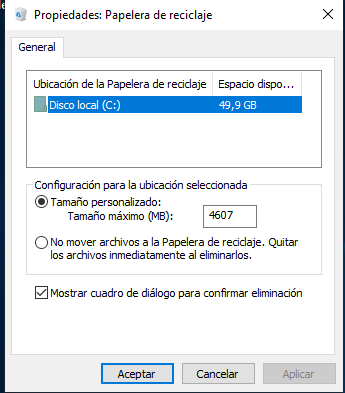
\includegraphics{png/PapeleraWS.png} El tancament de sessió i l'apagat
d'un servidor requereix més precaucions que en una estació de treball
(Windows 1x).

Respecte a l'\textbf{apagat del servidor}, aquets, solen estar executant
serveis crítics i aplicacions de xarxa. Apagar incorrectament un
servidor pot causar pèrdua de dades o interrupció del servei. El procés
d'apagat ha de ser planificat i queda registrada la causa que indiquem.

Respecte al \textbf{tancament de sessió}, l'estat normal deu ser amb la
sessió tancada excepte quan un administrador ha de fer alguna tasca. La
sessió deu estar el temps estrictament necessari i el login no deu estar
visible per raons de seguretat.

Per raons de seguretat, a banda d'evitar l'accès físic al servidor, cal
que només tinguem iniciada una sessió el temps justet per fer la tasca
de manteniment.

\end{document}
